%%%%%%%%%%%%%%%%%%%%%%%%%%%%%%%%%%%%%%%%%%%%%%%%%%%%%%%%%%%%%%%%%%%%%%%%%%%%%%%%%%%%%%%%%%
\section{Methods}

%%%%%%%%%%%%%%%%%%%%%%%%%%%%%%%%%%%%%%%%%%%%%
\subsection{Dataset} \label{sec:method_dataset} 

\begin{table}[H]
    \centering
    \caption{List of all features used in analysis. The exact feature
    definitions can be found in the appendix \ref{sec:appendix_feature_definitions}}  
    \label{tab:features} 
    \begin{tabular}{|c|c|}
        \hline
        Feature number & Feature name \\
        \hline
        0            & histogram max \\
        \hline
        1           & histogram mean \\
        \hline
        2            & histogram min \\
        \hline
        3           & histogram peak \\
        \hline
        4            & histogram std \\
        \hline
        5       & shape area\_density \\
        \hline
        6   & shape convex\_hull\_area \\
        \hline
        7            & shape surface \\
        \hline
        8             & shape volume \\
        \hline
        9     & shape volume\_density \\
        \hline
        10            & glcm cluster \\
        \hline
        11           & glcm contrast \\
        \hline
        12            & glcm entropy \\
        \hline
        13        & glcm homogeneity \\
        \hline
        14      & glcm joint\_maximum \\
        \hline
    \end{tabular} 
\end{table}



Our dataset contains 15 Radiomics features extracted on 16 different lymphom
cancers. All the feature values can be found in the Github repository (\url{https://github.com/jensjpedersen/Projects_FYS-STK4155/tree/main/Project3}) with path
\verb|./Data/big_test.csv|. The name column corresponds to the different tumors
(Volume of Interest's), the series column contains the names of a total of six
unique PET reconstruction methods. The analysis done in this report uses only
tree of the six reconstruction methods, with names PT\_PET\_EARL2,
PT\_PET\_EARLAC and PT\_PET\_WB\_Q\_CLEAR. They will be our target class
labels in or supervised classification methods. The respective feature names
can be found in the feature\_name column with it's respective values in the
value column.  

To read the data, the following python code can be used. 
\begin{lstlisting}[language=Python]
import read_csv
input_path = '../../Data/big_test.csv'
r = read_csv.ReadCSV(input_path)
r._remove_series([2, 3, 5])
X, y = r.get_df()
\end{lstlisting}
In the above code X is a pandas frame with size $n=3 \cdot 16$ rows (sample
size) and $p = 15$ columns (features). Our target class labels (reconstruction
methods) is encoded as a
on hot vector, where the first, second and third correspond to our
reconstruction methods 
PT\_PET\_EARL2  PT\_PET\_EARLAC  PT\_PET\_WB\_Q\_Clear respectively. In the
cases where integer class labels is used to reference the different target the
values 0, 1 and 2 are use in the respective order as above. 

The features are listed in table \ref{tab:features}. For exact feature
definitions see \ref{sec:appendix_feature_definitions}. All the features is
aggregated in a Volume Of Interest (VOI). Each VOI has a
threshold of $0.41 \cdot max$. 
That is, the minimum value in the VOI is larger or equal to 0.41\% of the
maximum value voxel (3D pixel) intensity in the tumor. Defining the boundary as a minimum
value is meaningful since the voxel intensity value in a PET scanner
is positively correlated with cell proliferation. 
All the images is acquired with a PET Scanner % XXX:type 
where different image reconstruction techniques was applied to each image. In our analysis we will study 3
different reconstruction methods. This will be our classification
targets. Thus, we are interested to see if it is possibly to identify features
that gives good class separation with respect to reconstruction method. This
will be a challenging since our data only contains 16 samples per
reconstruction. Hence, a total of $16 \cdot 3$ data points. 
This will be an exercise in selecting a few good features to prevent
overfitting applied to simple supervised classification models.   


\subsection{Decision Tree Classifier} \label{sec:method_descion_tree} 
A classification decision tree is a predictive model that predicts the target
class of a feature based on a set of binary rules. The decision tree consists of a series of
nodes, branches, and leaves. Each node represents a decision point, each branch
represents a possible outcome, and each leaf represents a final consequence or
result. 

% XXX: explain fig
% and structure in a decision tree
\begin{figure}[H]
    \centering
    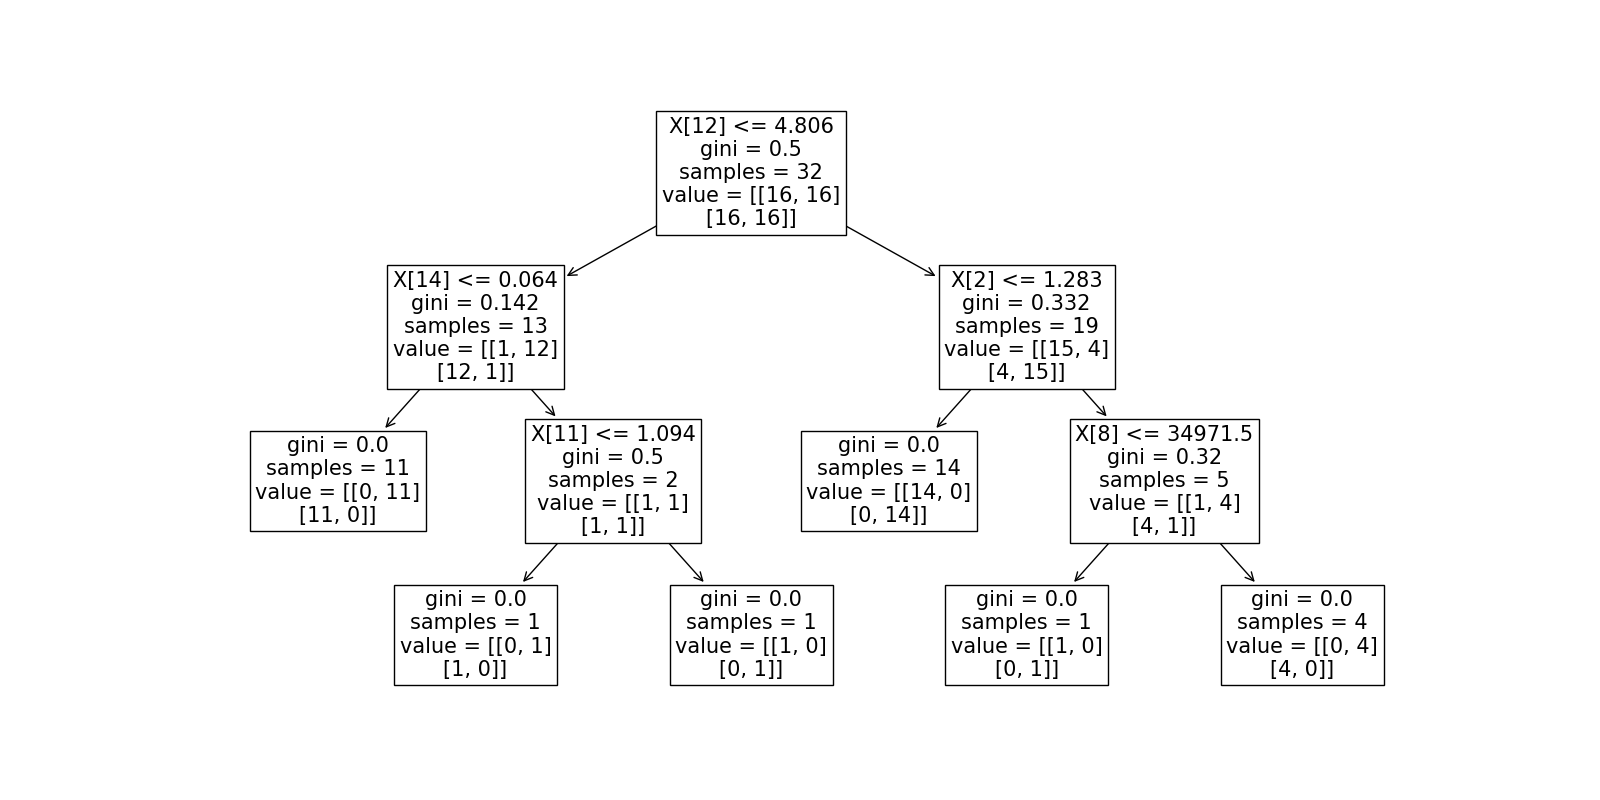
\includegraphics[width=0.8\textwidth]{Figures/descion_tree.png}
    \caption{Decision tree}  
    \label{fig:descision_tree} 
\end{figure}

A typical structure of a decision is shown in figure \ref{fig:descision_tree}. Each rectangle
represents a node in the tree. The build of a decision consists of finding
the feature and feature value (threshold) at each node that maximizes the
purity of each child node resulting from the split. At each node the data is
split into two child nodes based on the threshold value. Values lower than the threshold is
passed to the left child node and values higher is passed to the right child
node. Thus, the tree consists of a set of rules on where to place a specific sample. The algorithm is recursive and starts at the
root node (the upper rectangle) on continues until a Leaf node is reached.
That is, one of the squares in the bottom of the figures.     


\subsubsection{The CART algorithm} \hfill

We implemented the CART algorithm to find the optimal splits in the data.  

The CART algorithm splits the data set in two subsets using a single feature
$k$ and a threshold $t_k$ \cite{w44}. The purity of the split is then evaluated
with the cost function: 
\begin{equation*}
    \label{eq:cart} 
    C(k, t_k) = \frac{m_{\text{left}} }{m} G_{\text{left}}+
    \frac{m_{\text{right}} }{m} G_{\text{right}}, 
\end{equation*}

where $G$ is a measure of impurity (see section \ref{sec:gini_factor}),
$m_{\text{left}} $ and $m_{\text{right}} $ is the number of samples in the left
and right subsets resulting from the split. The total number of samples is $m =
m_{left} + m_{right}  $ 

The algorithm iterates through all p features and n samples. For each feature k
and threshod $t_k$, the cost score is evaluated on the two subsets. The
threshold and features that produced the best score is stored in a node. This
process is repeated on the data subsets in a recursive way until a specific
criterion is met. This produces a leaf node in the tree. 

In our implementation the recursion stops if it is not possible to split the
subset further. That is, the number of samples in the subset is equal to one.   
The recursion will also stop if our subset is 100\% pure. That is, the subset
only consist of one class label.  

\subsubsection{Gini factor} \label{sec:gini_factor} \hfill

The Gini factor is used to measure the purity of the data subset and is
calculated as:
\begin{equation*}
    G = 1 - \sum_{i=1}^{c} P_i ^2 
\end{equation*}
where $P_i$ is the probability that a sample belongs to class i. 

For a maximum impurity, where $P_1 = P_2 = 0.5$ the Gini factor is 0.5. A
smaller value indicates a more pure data subset. For a perfectly pure class the Gini
factor is 1. That is all the samples belongs to a class k ($P_k = 1$).     


Our class target labels was stored in one hot vector of size $n \times c$, 
where n is the number of samples in the data subset and c is the number of
classes. The probability of each class was calculated with this python snippet:
\begin{lstlisting}[language=Python]
import numpy as np
P = np.sum(y, axis = 0)/y.shape[0]
\end{lstlisting},
where \verb|y| is the one hot vector of our class targets. 

\subsubsection{Feature importance} \label{sec:feature_imporance} 
Our random forest implementation was used to identify most discriminative
features and not used for its predictive power. Again, we will use the Gini
factor to calculate the feature importance. 


We want to quantify the impurity decrease as results of a feature split.
Therefore, we are interested in the change in impurity with respect to a node and its
child nodes. The impurity decrease also needs to take into account the number
of samples. A feature is more important if it is able to separate more samples.       

% We will use the same formula as the scikit learn python library \cite{sklearn}
to estimate the feature importance: 
\begin{equation*}
    \frac{m}{M} \cdot (G  - \frac{m_{\text{left}} }{m} G_{\text{left}}+
    \frac{m_{\text{right}} }{m} G_{\text{right}}), 
\end{equation*}
where $G$, $G_{left} $ and $G_{right} $ as the Gini factor for the parent,
left child and right child node respectively. M is the total number of samples
in our input data. The other quantities are as defined in equation
\ref{eq:cart}. 

All our decision trees has a variable called \verb|feature_importances_|, which
contains the impurity decrease obtained from the best split of a node (except
for leaf nodes).   

When building the tree all features is considered each time a node is to be
split. If the same feature is used multiple times to split nodes in to a tree.
Then, only the split that produces the highest impurity decrease is stored in
the \verb|feature_importances_| variable. Hence, used to evaluate the feature
importance.      



Our decision tree algorithm can be used directly to identify good features.
However, there are some problems. The algorithm usually produces very different
results dependent on small variations in the data. That is, classification
decision trees suffers from high variance. It may also neglect highly
correlated features that produces a slightly poorer separation. To circumvent
these problems we implemented the random forest algorithm. 

%%%%%%%%%%%%%%%%%%%%%%%%%%%%%%%%%%%%%%%%%%%%%

\subsection{Random forest} \label{sec:method_random_forest} 
Random forest is a type of ensemble learning method, which uses multiple
decision trees to make predictions and combines them to create a more accurate
and stable prediction. 

In our first attempt to identify good features (features with good
class separation), we will use a random forest classifier. 
It can be used to identify the features and feature value that splits the data
into the purest classes (see section \ref{sec:feature_imporance})
The algorithm works by constructing multiple decision trees, each of which is trained 
on a subset of the data. 

It uses a technique called bagging, which involves
randomly selecting a subset of data from the training set and building a
decision tree from each subset. 

It also uses feature resampling to reduce the
overfitting of the model. We will implement feature resampling
to better evaluate the performance of all the features. Feature resampling is
done within each node of the descion tree. Hence, the best split at each node is
evaluated on different feature subsets. The pseudocode for building a random
forest is shown in Algorithm \ref{alg:random_forest}. The algorithm is reused
from \cite{w44}.  


\begin{algorithm}
\caption{Growing a Random Forest} \label{alg:random_forest} 
\begin{algorithmic}[1]
\State {\bfseries Input:} training data $\boldsymbol{X}$, number of trees $B$
\State Initialize forest $\bm{T} \gets {}$
\For{$b \gets 1$ {\bfseries to} $B$}
\State Draw a bootstrap sample from $\boldsymbol{X}$
\State Initialize tree $T_b$
\While{node size $<$ maximum}
\State Select $m \leq p$ random variables from $p$ predictors/features
\State Select best split point among $m$ variables using CART algorithm
\State Create new node and split into daughter nodes
\EndWhile
\State Add tree $T_b$ to forest $\bm{T}$
\EndFor
\State {\bfseries Output:} ensemble of trees $\bm{T}$
\end{algorithmic}
\end{algorithm}


% \paragraph{Algorithm} 

% % Random forest algorithm - cite lecture 44
% \fbox{\begin{minipage}{30em}
% We will grow of forest of say $\bm{B}$ trees.

% For b=1:B

% Draw a bootstrap sample from the training data organized in our $\boldsymbol{X}$ matrix.

% We grow then a random forest tree $T_b $
% based on the bootstrapped data by repeating the steps outlined till we reach
% the maximum node size is reached

% we select $m \leq p$  variables at random from the p predictors/features

% pick the best split point among the $m$ features using for the CART
% algorithm and create a new node

% split the node into daughter nodes

% Output then the ensemble of trees $\{T_b\}^B_1$

% and make predictions for either a regression type of problem or a
% classification type of problem.
% \end{minipage}}

% Discuss differences with own implementation and sklearn

We did compare our own implementation of the random forest to the python
scikit learn function RandomForestClassifier. For sklearn and our own
implementation we used the following parameters, \verb|n_estimators=100000|,
\verb|max_features='sqrt'|. Where n\_estimators is the number of decision trees
in the forest. A total of $\sqrt{p} $ random features was considered in each
split, where p=15, is the total number of features. Then the models was fitted
to the full dataset. Our fitted classifier will then contain a list of all the
fitted decision trees. The feature\_importances\_ variable obtained from all the
decision trees was used to find the overall best features.  

The results from our own implementation and sci-learn was in perfect agreement
with respect to ranking feature importance. 
However, the impurity decrease obtained with sklearn was
approximately two times larger for all features compared with the results obtained with our own
implementation. Our own implementation was also more tan 100 times slower
compared to
sklearn. An increase in runtime from minutts to hours. This defeats the purpose
of our feature selection algorithm. 
Therefore, the results obtained with the random forest in table
\ref{tab:feature_importance}  is obtained with sklearn's implementation. 
The following python code can easily
be used to reproduce our results:  
\begin{lstlisting}[language=Python]
import numpy as np 
from sklearn.ensemble import RandomForestClassifier
np.random.seed(0)
RandomForestClassifier(n_estimators=10000, max_features='sqrt')
clf.fit(X, y)
importances = np.zeros((clf.n_estimators, X.shape[1]))
for i, tree_clf in enumerate(clf.estimators_): 
    importances[i, :] = tree_clf.feature_importances_
importances = np.mean(importances, axis = 0)
\end{lstlisting}
The mean importance decrease of all the features was stored in the importances
variable. The results obtained with our own implementation is listed in table
\ref{tab:feature_importance_own} in the appendix. 
% explain elements in code






















% What is one hot vector?
% A one hot vector is a vector of all zeros, except for a single element which is set to one. 
% It is commonly used to represent a categorical variable in machine learning models.





%%%%%%%%%%%%%%%%%%%%%%%%%%%%%%%%%%%%%%%%%%%%%
\subsection{Pearson correlation}
Pearson correlation is a statistical measure of the linear relationship between
two variables. It is used to assess the strength and direction of the
relationship between two continuous variables.
The Pearson correlation coefficient ranges from -1 to 1, with values closer to
1 indicating a strong positive relationship, values closer to -1 indicating a
strong negative relationship, and values closer to 0 indicating a weak or no
relationship.

To evaluate the correlation between features we used the 
\verb|pandas.DataFrame.corr| functionality from the Pandas python package. We
only considered highly positively correlated features when looking for
redundant features.   

















\subsubsection{SVM}
Support Vector Machine (SVM) is a machine learning method used for 
classification and regression problems. We will use SVM for binary 
classification where the algorithm's aim is to create a $p-1$ dimensional
affine subspace of the $p$ dimensional feature space which distinguishes all the 
classifications optimally. This subspace is called a hyperplane and the 
optimal hyperplane maximizes the margin which is the distance from the 
hyperplane to the nearest data point in feature space. The optimal hyperplane 
will therefore be the same distance from the nearest point(s) of each 
classification it divides. These points are called the support vectors.

The hyperplane is defined by a $p$ dimensional weight vector $\boldsymbol{w}$ and a 
bias term $b$
\begin{equation}
\boldsymbol{x^T}\boldsymbol{w} + b =0, 
\label{eq:hyperplane}
\end{equation}
where $\boldsymbol{x^T}=[x_1,x_2,...,x_p]$ is the transpose of a point in feature space.
Separating our classifications by $y_i=1$ or $y_i=-1$, we can classify a 
data point $x_i$ with our hyperplane as 
\begin{gather*}
y_i = sign(\boldsymbol{w^T}\boldsymbol{x_i}+b). 
\end{gather*}
Our margin defined by our hyperplane and training points $x_i$ with classification $y_i$ becomes the largest $M$ such that 
\begin{gather}
\frac{1}{||\boldsymbol{w}||}y_i(\boldsymbol{w^Tx_i}+b) \ge M, \forall i=1,2,...,p. 
\end{gather}
If we scale this equation such that $||\boldsymbol{w}||=1/M$, finding the maximal margin 
will be equivalent to minimizing 
\begin{gather*}
||\boldsymbol{w}||
\end{gather*}
subject to the constraints 
\begin{gather*}
y_i(\boldsymbol{w^Tx_i}+b) \ge 1, \forall i.
\end{gather*}

The optimization of the hyperplane can be solved using Lagrange multipliers. 
For each constraint formulated as $\phi_k (\boldsymbol{x})=0$, we add a Lagrange
multiplier $\lambda _k \ge 0$ such that $\frac{\partial f}{\partial x_i}+\lambda_k \frac{\partial \phi }{\partial x_i}=0$,
where $f(\boldsymbol{x})$ with $x_i \epsilon [\boldsymbol{x}]$ is the function we want to minimize 
subject to the constraints.

Using the Lagrange multipliers, the optimization problem can be solved by minimizing 
the following Lagrangian function
\begin{equation}
	L(\lambda ,b,\boldsymbol{w})=\frac{1}{2}\boldsymbol{w^Tw}-\sum_{i} \lambda _i[y_i(\boldsymbol{w^Tx_i}+b)]-1,\lambda _i \ge0. 
	\label{eq:Lagrangian}
\end{equation}
Taking the derivatives with respect to $\boldsymbol{w}$ and $b$ we obtain the constraints 
\begin{gather*}
\frac{\partial L}{\partial b}=-\sum_{i} \lambda _i y_i=0,
\quad \frac{\partial L}{\partial \boldsymbol{w} }= \boldsymbol{w} -\sum_{i} \lambda _i y_i \boldsymbol{x_i} =0.
\end{gather*}
Inserting these constraints in \autoref{eq:Lagrangian}, we are able to get rid 
of the variables $\boldsymbol{w}$ and $b$ from the Lagrangian
\begin{equation}
L = \sum_{i} \lambda _i - \frac{1}{2}\sum_{ij}^{n} \lambda _i \lambda _j y_i y_j \boldsymbol{x_i^Tx_j},
\label{eq:Lagrangian_lmb}
\end{equation}
with constraints $\lambda _i \ge 0$ and $\sum_{i} \lambda _iy_i=0$.
Additionally, the Karush-Kuhn-Tucker condition has to be satisfied
\begin{gather*}
\lambda _i >0 \implies y_i(\boldsymbol{w^Tx_i}+b)=1, \quad y_i(\boldsymbol{w^Tx_i}+b)>1 \implies \lambda _i = 0,
\end{gather*}
such that $\lambda _i>0$ if and only if $\boldsymbol{x_i}$ is a support vector. 

There is often overlap between classifications in feature space. Then, there 
won't exist a hyperplane able to separate all the classifications. We will 
implement two ways to deal with this problem. 

The first is to introduce slack variables. The slack variables 
$\varepsilon _i \ge  0$ allows for some misclassification of 
the training data. The amount of misclassification is governed by the 
slack constant $C$ which sets a bound on the sum of the slack variables.  
Utilizing this method turns our SVM in to a so-called soft classifier as 
opposed to a hard classifier. 
The Lagrangian stays the same as \autoref{eq:Lagrangian_lmb}, but 
with different constraints:
\begin{gather*}
	\sum_{i} \lambda _i y_i = 0, \quad 0 \le \gamma _i \le C,\\
	\lambda _i[y_i(\boldsymbol{w^Tx_i}+b)-(1-\varepsilon _i)]=0,\\
y_i(\boldsymbol{w^Tx_i}+b)-(1-\varepsilon _i) \ge 0.
\end{gather*}

The second method is to transform the basis of the feature space to obtain 
better separation between classifications. This is done with a so-called 
kernel $K$ which transforms the data in \autoref{eq:Lagrangian_lmb} by 
\begin{gather*}
\boldsymbol{x_i^Tx_j} \rightarrow ø(\boldsymbol{x_i})^Tø(\boldsymbol{x_j})=K(\boldsymbol{x_i,x_j}),
\end{gather*}
where $ø(\boldsymbol{x})$ is some transformation of the feature space.

Our Lagrangian in \autoref{eq:Lagrangian_lmb} expressed as a convex optimization 
problem in terms of a matrix equation using a kernel $K$ may be written as 
\begin{equation}
\frac{1}{2}\boldsymbol{\lambda ^T}
\begin{bmatrix}
	 y_1y_1K(\boldsymbol{x_1,x_1})  & y_1y_2K(\boldsymbol{x_1,x_2}) & \hdots & y_1y_nK(\boldsymbol{x_1,x_n}) \\
	 y_2y_1K(\boldsymbol{x_2,x_1})  & y_2y_2K(\boldsymbol{x_2,x_2}) & \hdots & y_2y_nK(\boldsymbol{x_2,x_n}) \\
	\vdots & \vdots & \ddots & \vdots \\
	 y_ny_1K(\boldsymbol{x_n,x_1})  & y_ny_2K(\boldsymbol{x_n,x_2}) & \hdots & y_ny_nK(\boldsymbol{x_n,x_n}) \\
\end{bmatrix}
\boldsymbol{\lambda }-\mathbb{1}\boldsymbol{\lambda },
\label{eq:Lagrangian_mateq}
\end{equation}
where $\mathbb{1}=[1,1,...,1]$ is $n$ dimensional. Here $\boldsymbol{\lambda }=[\lambda _1,\lambda _2,...,\lambda _n]^T$ 
and $\boldsymbol{y}=[y_1,y_2,...,y_n]^T$. The constraints can be written as 
$\boldsymbol{y^T\lambda }=0$, and $0 \le \lambda _i \le C$ assuming we are using 
a slack constant $C$.  

There are many popular kernels such as the Gaussian radial basis function which 
we will use:
\begin{equation}
K(\boldsymbol{x_i,x_j})=exp(-\gamma ||\boldsymbol{x_i-x_j}||^2).
\label{eq:grbf}
\end{equation}
Here, $\gamma $ is a constant which needs to be tuned.
We know that the feature space transformation $ø$ defining the kernel exists based 
on Mercer's theorem which states that if $K$ is symmetric, continuous and leads to 
a positive semi-definite matrix $P$ defined in \autoref{eq:Lagrangian_mateq}, then 
$ø$ exists. 

To minimize \autoref{eq:Lagrangian_mateq}, we will use \verb|solvers.qp| from
the python library \verb|cvxopt|. The solver takes the minimization problem 
and its constraints as matrix equations:
\begin{equation}
	\begin{split}
		\text{min}_{\boldsymbol{\lambda }}\quad \frac{1}{2}\boldsymbol{\lambda ^TP\lambda +q^T\lambda },\\
	\text{subject to}\quad \boldsymbol{G \lambda  \le h}, \quad \boldsymbol{A \lambda =b}.
	\end{split}
	\label{eq:solver_eq}
\end{equation}

The problem in \autoref{eq:solver_eq} are defined and solved based on \autoref{eq:Lagrangian_mateq}
in the following code:
\begin{lstlisting}[language=Python]
def solve(self):
        # Solution for minimizing 
        # (1/2) * lambda.T @ P @ lambda + q.T @ lambda 
        # subject to constraints

        y = self.y_train
        X = self.X_train
        n = self.X_train.shape[0]

        q = -1 * np.ones(n).T
        P = np.zeros((n, n))
        for i in range(n):
            for j in range(n):
                P[i,j] = y[i] * y[j] * self.K(X[i,:], X[j,:])
        
        # G and h sets constraints on col vec lambda: G@lambda <= h
        G = np.zeros((2*n, n))
        G [:n, :] = np.identity(n) * (- 1)
        G[n:,:] = np.identity(n)
        h = np.zeros(2*n)
        h[n:] = np.ones(n) * self.C
        # A and b sets  constraints on labda: A@lambda = b
        A = np.array(self.y_train, dtype=float).T
        b = np.zeros(1) 
    
        # Solve 
        P, q, G, h, A, b = matrix(P), matrix(q), matrix(G), matrix(h), matrix(A), matrix(b)
        solvers.options['show_progress'] = False
        sol = solvers.qp(P, q, G, h, A, b)
        self.lmb = np.array(sol["x"])
        self.lmb_non_zero_indecies = np.where(self.lmb > 1e-5)[0]
        self.calc_b()
\end{lstlisting}

Having obtained our Lagrange multipliers, we are able to calculate our bias term 
\begin{gather*}
b = \frac{1}{N_s}\sum_{j\epsilon N_s} (y_j-\sum_{i=1}^{n} \lambda _i y_i K(\boldsymbol{x_i,x_j}),
\end{gather*}
where $N_s$ is the number of support vectors with indices $j$.
Then, we are able to predict the classification of a point $x_i$ in feature space by 
\begin{gather*}
y_i = sign(b + {N_s}\sum_{j\epsilon N_s} y_j \lambda _j K(\boldsymbol{x_i,x_j})
\end{gather*}


%%%%%%%%%%%%%%%%%%%%%%%%%%%%%%%%%%%%%%%%%%%%%
\subsection{Cross Validation}
We will use k-fold cross validation with multiple cycles to increase the
precession of the test accuracy score. 
%Section is a bit short but don't know what else to write
The steps of k-fold cross-validation is:
\begin{mdframed}[backgroundcolor=black!10]
\raggedright

1. Shuffle the dataset randomly.\\

2. Split the dataset into $k$ groups.\\

3. For each unique group:\\

\hspace{1cm}a. Decide which group to use as a set for test data\\

\hspace{1cm}b. Take the remaining groups as a set for training data\\

\hspace{1cm}c. Fit a model on the training set and evaluate it on the test set\\

\hspace{1cm}d. Retain the evaluation score and discard the model\\

5. Summarize the model using the sample of model evaluation scores\\

\end{mdframed}

%close to lecture notes XXX: cite lec notes
The advantage of cross-validation is that the data splitting is not done
randomly so we don't get any unwanted influence on the model building or
prediction evaluation. This is called a  $k$-fold cross-validation structures
the data splitting involves dividing the samples $k$ more or less equally sized
exhaustive and mutually exclusive subsets. In turn (at each split) one of these
subsets plays the role of the test set while the union of the remaining subsets
constitutes the training set. Such a splitting warrants a balanced
representation of each sample in both training and test set over the splits. 

Multiple cycle cross-validation is a variant of cross-validation that involves
repeating the process multiple times, each time using a different combination
of the data as the training and evaluation sets. 

